%% ==============================
% Part is used only in PhD thesis
\part{The Implementation}
\chapter{\iflanguage{ngerman}{Implementierung}{Implementation}}
\label{sec:implementation}
%% ==============================
In this Chapter the details of the experimental process will be specifically introduced. According to the pipeline introduced in the previous section, the experiment is mainly divided into 3 parts, the model optimization, rendering optimization and method optimization by using multiple camera as input data. Section 5.1 specifies the process and result of model optimization, which is based on simulation data implemented. Section 5.2 describes the process, that we train the models with images rendered by different simulation conditions, and verify the performance of the models in real world, which aims to analyze the impact of different rendering conditions to get a best rendering environment. The section 5.3 aims to improve the recognition accuracy by using further optimization method, here the multi-camera system are used in our experiment to explore whether the recognition accuracy can be improved by increase the information inputs.

\section{Scene Setup}
Building the experiment scene is the first step of our work. Aiming to train the detector for pose estimation of object in simulation environment, we first need to construct the scene in real world, which is the basis of simulation. 

\subsection{Scene in Real World}
The experiment scene for pose estimation is set on the workbench of \textit{Franka Emika Panda}\footnote{https://www.franka.de/panda/}. Within a thing pad on the table the objects are located, which are expected to be detected in the experiment. Camera is placed at the end effector of the robot. A initial distance of 50 cm is set from the camera to table. Each time the images will be captured from the initial position. We did not control for lighting conditions or the rest of the scene around the table. The scene built is shown in figure5:

\missingfigure{}

\subsection{Scene in Simulation}
After the scene is built in real world, we create the corresponding models in Unity3D. The architectural relationship will be rebuild in  simulation environment. Then we add ambient light into the scene to simulate realistic lighting conditions. The required function modules are also added into the scene for rendering different images. The simulated scene is shown in figure 5

\missingfigure{}

\section{Model Optimization}
The models used in the experiments were modified VGG-16, ResNet-50 and Inception-v3 networks, which are described in Chapter 4. The main purpose of this part of experiment is to compare the performance of these three base models and then modify the structure and hyperparameters of the model with best performance on our task. The optimized model can be used in further experiment. 

\subsection{Base Model}
We chose VGG-16, ResNet-50 and Inception-v3 as candidate base models for our experiment, because they all have good performance in image process tasks in the field of computer vision. Firstly, we need to select one model with best performance on our 3D pose estimation task from these three. \author{\textit{\{Canziani, Alfredo and Paszke, Adam and Culurciello, Eugenio}} in \cite{canziani2016analysis} analyzed the performance of different deep neural network models for practical applications. Figure 5.1 shows Inception-v3 hat the best Top-1 accuracy in these three models, and ResNet-50 performs better than VGG-16. The amount of operations required for a single forward pass of different models are shown in figure 5.2. The parameters of Inception-v3 and ResNet-50 are significantly less than VGG-16, so they consume less computation in training process and have higher efficiency. By comparison, it can be concluded that the performance of the Inception-v3 is better than the other two networks in terms of Top-1 accuracy and training efficiency. 

\begin{figure}[h]
	\centering
	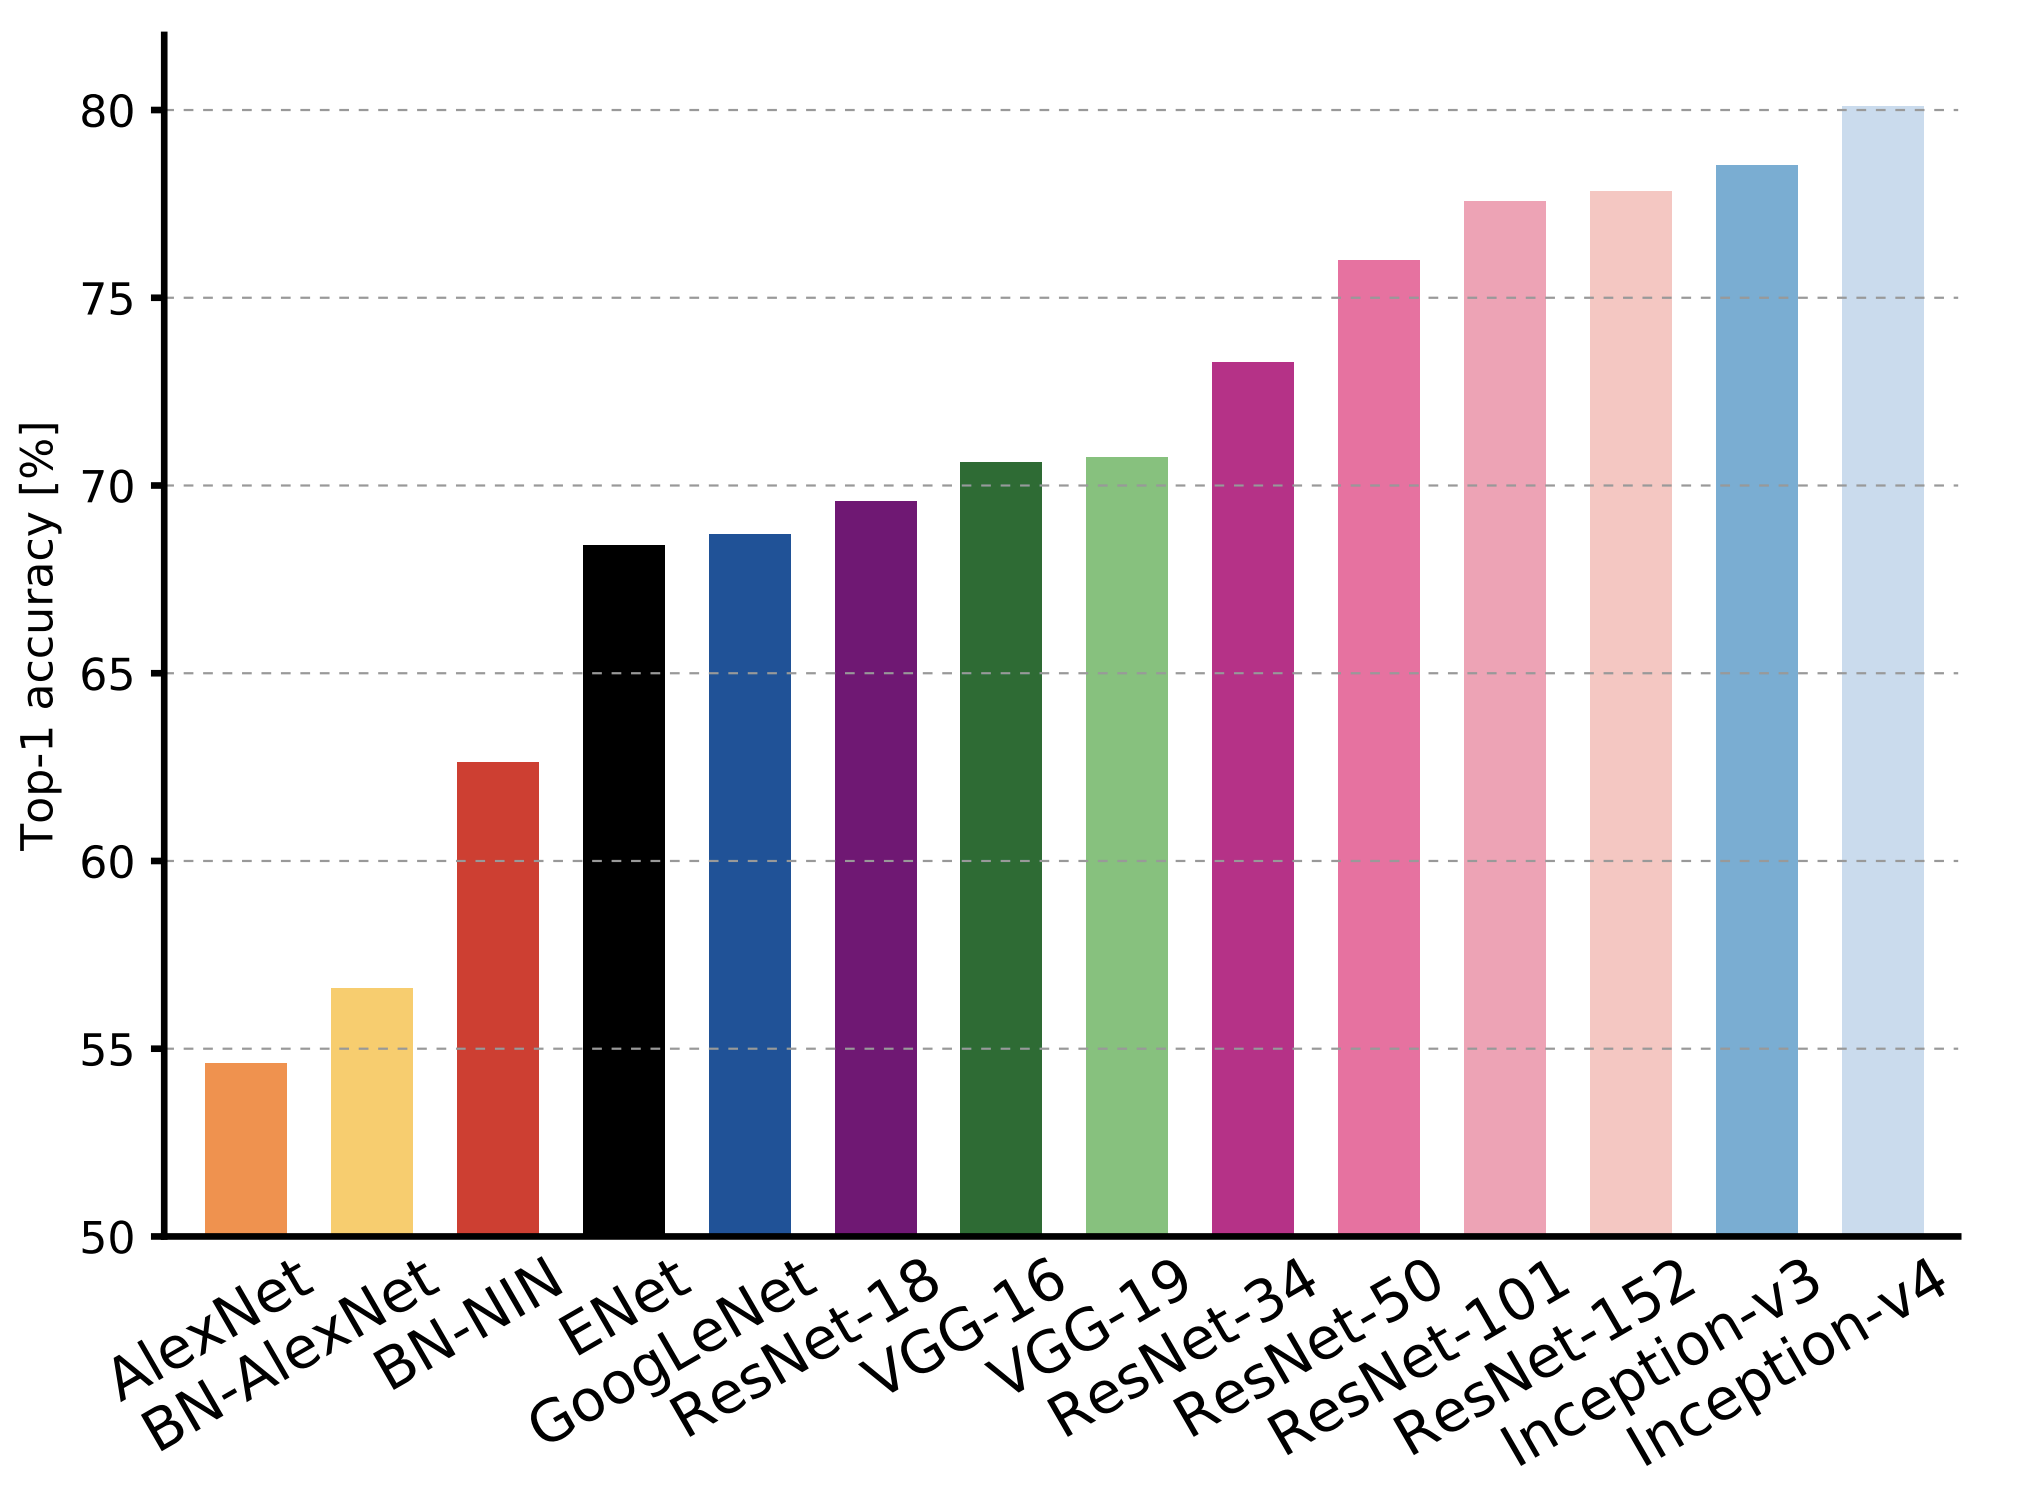
\includegraphics[width=0.7\textwidth]{Figures/Section5_Top1_acc_1}
	\caption{\textbf{Top1 \textit{vs.} network.} Single-crop top-1 validation accuracies for top scoring single-model architectures.\cite{canziani2016analysis} }
	\label{fig:Top1_1}
\end{figure}
\begin{figure}[h]
	\centering
	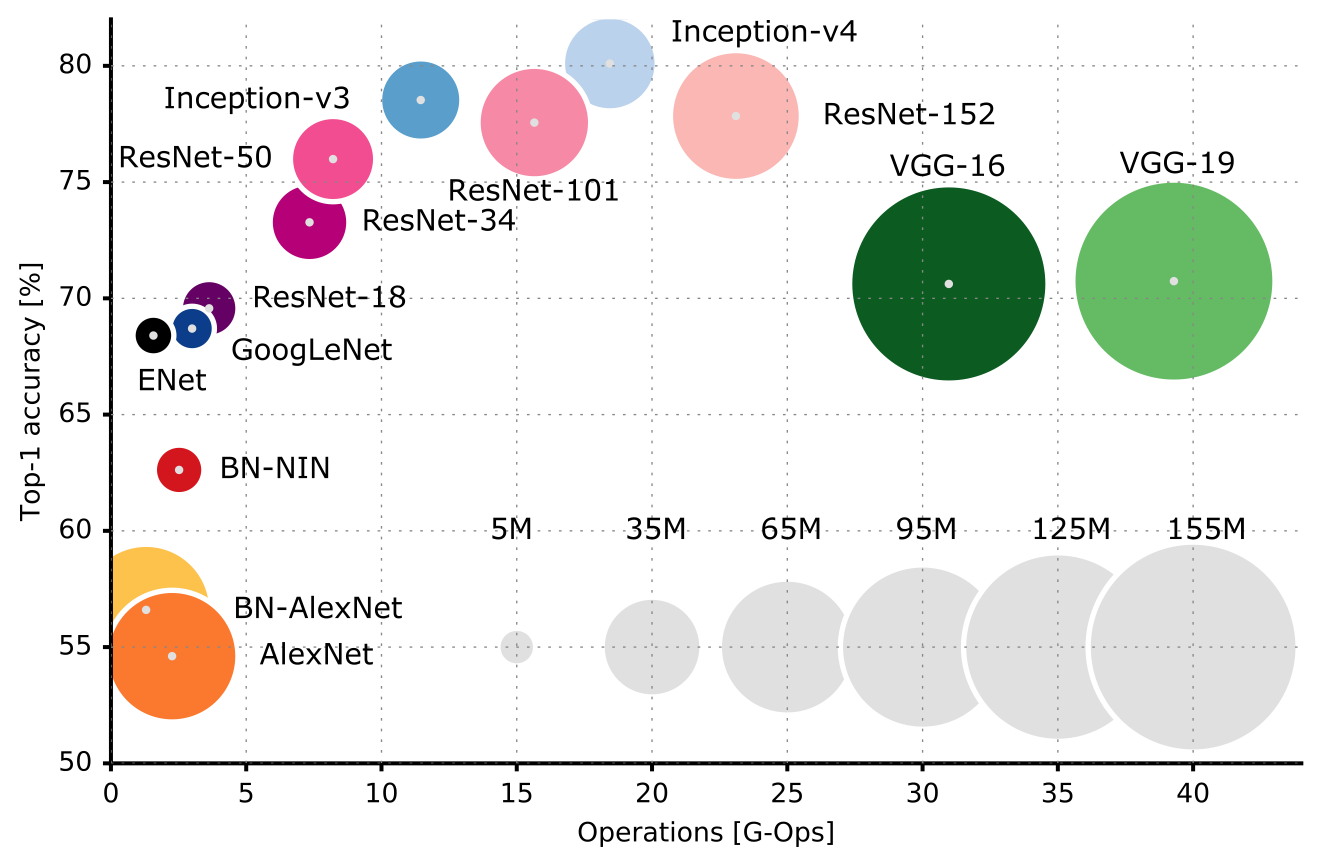
\includegraphics[width=0.7\textwidth]{Figures/Section5_Top1_acc}
	\caption{\textbf{Top1\textit{vs.} operations, size $\propto$ parameters.}Top-1 one-crop accuracy versus amount of operations required for a single forward pass.\ The size of the blobs is proportional to the number of network parameters; a legend is reported in the bottom right corner, spanning from $5\times10^{6}$ to $ 155\times10^{6} $ params.  Both these figures share the same $y$-axis, and the grey dots highlight the centre of the blobs. \cite{canziani2016analysis}} 
	\label{fig:Top1_2}
\end{figure}


Next, we will verify the performance of the three models on our 3D pose estimation task, and demonstrate whether the results are consistent with \cite{canziani2016analysis}. Then the model with best performance will be selected for further experiments. In this experiment, the three models will be set to the same hyperparameters while keeping the structure of the convolutional layers unchanged, and the fully connected layers will be downsized to 256. The table 5.1 shows the summary of the hyperparameters used in this experiment.

\begin{table}[]
	\begin{tabular}{c|c|c|c|c}
		\hline
		\textbf{Fully connected layers size} & \textbf{Batch size} & \textbf{Learning rate} & \textbf{Learning rate decay} & \textbf{Epochs} \\ \hline
		256                                  & 32                  & 0.0001                 & 0                            & 60              \\ \hline
	\end{tabular}
	\caption{Hyperparameters use to verify performance of VGG-16, ResNet-50 and Inception-v3 }
	\label{table:Compare_basemodel}
\end{table}

\textbf{Result}
\missingfigure{}

In figure 5.4, the validation loss of different modified models can be seen. From the results in the figure we find that the validation loss of the modified Inception-v3 is finally smaller than the other two models, that is, the error of the pose estimation is smaller and the accuracy is higher.  This conclusion is consistent with the analysis in \cite{canziani2016analysis}, so we will use Inception-v3 as the base model for the further experiment.

\subsection{Hyperparameters of Model Structure}
The goal of structure optimization is to improve the accuracy of our detector by modifying the model structure. According to the result from previous section, a modified Inception-v3 is set as the initial structure of our model, which is shown in figure 5.3. In the experiment the standard convolutional layers of Inception-v3 will be used, that means we don't change the structure of these layers. However, we change the size of the fully connected layer and 
remove Dropout after the average pooling layer.

All the hyperparameters will be set as the same in each modified structure, which are summarized in table 5.2. For the size of fully connected layer, we choose 64, 128, 256, 512 as the candidate parameters, and train the model with different sizes separately. And we analyze the performance of different models on the validation set of simulation data.

\begin{table}[]
	\begin{tabular}{c|c|c|c}
		\hline
		\textbf{Batch size} & \textbf{Learning rate} & \textbf{Learning rate decay} & \textbf{Epochs} \\ \hline
		32                  & 0.0001                 & 0                            & 60              \\ \hline
	\end{tabular}
\end{table}

Here the validation loss and mean absolute error are used to evaluate the results. Both values represent the error between the predicted pose and the real pose. The mean absolute error describes the average error as mentioned before. However, the loss function is based on $L2 loss$ (mean squared error), which is more sensitive to outliers, so we combine both results to judge the performance of the model. That means, the smaller the result of these two values, the better the performance of the model.

\textbf{Result}

After training, we obtain the curve of validation loss and mean absolute error as shown in figure 5.4. The $x$-axis indicates the training epochs, and the $y$-axis indicates the corresponding validation loss and MAE.

\missingfigure{}

It can be seen from the curve variation in the figure that the model trained with size of 256 for the fully connected layer performs best. The validation loss and MAE are smaller than those of other size. That means, the model has a smaller average error, and the distribution of errors is more concentrated \footnote{Since the hyperparameters are not set to be optima at this time, and the training set is not rendered with the best rendering conditions, both the validation loss and MAE are larger than the final result.}. 


\subsection{Hyperparameters of Training Process}
In this section we aim to select the appropriate hyperparameters to optimize the training process. According to the experiments in the previous sections, the modified Inception-v3 was chose for hyperparameter tuning, because it has a better performance for our pose estimation task.

The main hyperparameters of this part include learning rate, learning rate decay, batch size and epochs. We try to select larger batch size in the early stage of the experiment to make full use of the graphics resources and improve the convergence speed. By tuning the learning rate and decay, the training result can converge quickly and avoid local optimal. And a appropriate epoch can prevent underfitting and overfitting.

We perform the experiment by evaluating combinations of different learning rates, decay and batch size. We divide the experiment into two steps. The first step is to select the best performing combination of learning rate and decay under the same batch size setting. Then different batch sizes can be examined based on the selected learning rate and decay to determine the batch size with best performance.

\subsubsection*{Learning rate and Decay}
The types of combinations we designed are shown in table 5.5.


\textbf{Result}\\
The models are trained based on the combination of parameters above. Figure 5.5 shows the training results.
\missingfigure{add}

\todo It can be seen from the figure that the model performs best when the learning rate is set to $0.001$ and the decay to $0.001$.

\subsubsection*{Batch size}
The types of combinations we designed are shown in table 5.6.

\textbf{Result}
We train the model with different batch sizes and get the results shown in figure 5.4.
\missingfigure{}


When batch size is set 8, the model will diverge and can not converge because the batch size is too small. When the batch size is 16 or 32, the model converges quickly and performs better, which gain the smaller error of the pose estimation. With the further increasing batch size the convergence of the model is slightly worse until 50 and 64. Based on the results above, we set the batch size to 32. In the case of ensuring better convergence of the model, the larger batch size can make full use of the graphics resources and improve the training efficiency.

\section{Rendering Optimization}
In the section we will generate die simulation scenes under different rendering conditions and use these data to train the models separately. The models will be then examined in the real world to evaluate the effects of these different rendering conditions. As mentioned in the previous chapter, we render the scenes with the method of domain randomization. The aspects of domain include:

\begin{itemize}
	\item Number and shape of distractor objects on the table
	\item Position and texture of all objects on the table
	\item Textures of the table, floor, skybox, and robot
	\item Position, orientation, and field of view of the camera
	\item Number of lights in the scene
	\item Position, orientation, and specular characteristics of the lights
	\item Type and amount of random noise added to image
\end{itemize}

\subsection{Pre-analysis}
It can be seen that the range of randomized domains here is large, many aspects may affect the performance of the final training result. In order to simplify the research, we selected several aspects of domain in our experiment, which we hypothesize may have a great influence on the training results. The selected aspects of the domain are summarized in table 5:

\begin{table}[h]
	\begin{tabular}{cl}
		\textbf{Num.} & \textbf{Selected aspects of the domain} \\
		1             & Additional textures on objects          \\
		2             & Color mode on objects                   \\
		3             & Additional textures on Environment      \\
		4             & Random noise                           
	\end{tabular}
\end{table}

We generate different rendered scenes with combination of the selected aspects of domain. The rest aspects of the domain are rendered full randomly in each sample, such as the position and number of the lights and the number of distractor objects, etc. Table 5.5 shows the combination of different rendering conditions.
\begin{table}[]
	\begin{tabular}{ccccc}
		\textbf{Evaluation Type Num.} & \multicolumn{1}{l}{\textbf{Color mode on target object}} & \multicolumn{1}{l}{\textbf{Addition textures on objects}} & \multicolumn{1}{l}{\textbf{Additional textures on Environment}} & \multicolumn{1}{l}{\textbf{Random noise}} \\
		1 & Full randomly & On & On & On \\
		2 & Full randomly & On & On & Off \\
		3 & Full randomly & Off & On & Off \\
		4 & Full randomly & Off & Off & Off \\
		5 & Around real color & On & On & On \\
		6 & Around real color & On & On & Off \\
		7 & Around real color & On & Off & On
	\end{tabular}
\end{table}

For the target object it can be set whether to perform a full random rendering, or render it around the real color. It can also be set whether to add additional complex textures on the object and to the environment, or they will be rendered in solid color. Here the environment includes the items in the scene except the target object and distractor objects, such as tables, floor and etc. The rendered images can be added with additional noise.


\subsection{Scene Rendering}
Each type of scenes can be rendered in Unity3D. With the functional modules we wrote in Unity3D, the rendering conditions can be controlled to generate the target scenes for the model training. All the  types of rendered scenes are shown in figure 5.5:
 \missingfigure{}
 
 Each column in the figure corresponds to a target scene. For each scene, the images for two cameras with different perspectives are captured for further experiments. The different rendering conditions between images in figure can be observed. For scene with additional complex texture, the generated images contains more information than those rendered with solid colors. We assume that the scene with texture more capable of simulating the complex real world. 
 
\subsection{Model Training}
The models will be trained by using the images from different rendered scenes. In the experiment, two types of target object are selected for our task, namely the cube and piston rod. The geometry of cube is relatively simple while the piston rod is more complexly constructed. By comparing the detection accuracy on these two objects, the influence of the complexity of the object shape on the training results. The model of the two objects is shown in figure 5.5:

\missingfigure{}

Through previous work, the model structure and it's hyperparameters are determined for a better training result. In the next experiment these parameters will be used for model training, which are summarized in table 5.5.

\begin{table}[]
	\begin{tabular}{|c|c|}
		\hline
		\multicolumn{2}{|l|}{\textbf{Determined hyperparameter for rendering optimization}} \\ \hline
		Base model & Inception-v3 \\ \hline
		Size of fully connected layer & 256 \\ \hline
		Optimizer & Adam \\ \hline
		learning rate & 0.001 \\ \hline
		Decay & 0.001 \\ \hline
		Batch size & 32 \\ \hline
		Epochs & 60 \\ \hline
	\end{tabular}
\end{table}

\subsection{Result}
The models trained in different rendered scenes will be evaluated in real world. We acquired 300 real data for the pose evaluation of the piston rod, of which in 200 data the distractor objects don't appear and the other 100 data contained the distractor objects with random shape and number. We use the model trained in different scenes to predict the 3D pose of rod piston, and calculate the prediction error. Following results were obtained: 

\begin{table}[]
	\begin{tabular}{|c|c|c|c|c|c|c|}
		\hline
		\multicolumn{7}{|c|}{\textbf{Detection error for Rod on real images}} \\ \hline
		\multirow{2}{*}{\textbf{Evaluation Type Num.}} & \multicolumn{3}{c|}{\textbf{Target object only}} & \multicolumn{3}{c|}{\textbf{Random noise}} \\ \cline{2-7} 
		& Position error & Rotation error & Total error & Position error & Rotation error & Total error \\ \hline
		1 &  &  &  &  &  &  \\ \hline
		2 &  &  &  &  &  &  \\ \hline
		3 &  &  &  &  &  &  \\ \hline
		4 &  &  &  &  &  &  \\ \hline
		5 &  &  &  &  &  &  \\ \hline
		6 &  &  &  &  &  &  \\ \hline
		7 &  &  &  &  &  &  \\ \hline
	\end{tabular}
\end{table}

Table II examines the performance of the algorithm under different rendered scenes. By comparing the result of set 1 and set 2 we found that rendering the target object around the real color is beneficial to improve the prediction accuracy. From the results of set 6 and 7, it can be seen that adding additional texture to the target object can also improve the performance of our model, and the model is more robust to the variations of scenes. The accuracy of the prediction is guaranteed to a good level when there are distractor objects in real scene. Similarly, adding additional textures to the environment has the same effect, the model can detect and estimate the pose of target object more accurately. Adding additional random noise did not improve the performance of the model in real world. We consider that by rendering complex lighting conditions and adding background textures, the complexity of the image information is high enough. Various noises are already included, so adding additional noise does not bring a significant improvement for the detection.
 
\begin{table}[]
	\begin{tabular}{|c|c|c|c|}
		\hline
		\multicolumn{4}{|c|}{\textbf{Detection error from best rendered scene}} \\ \hline
		\textbf{Evaluation types} & \textbf{Position error} & \textbf{Rotation error} & \textbf{Total error} \\ \hline
		Piston rod &  &  &  \\ \hline
		Cube &  &  &  \\ \hline
	\end{tabular}
\end{table}

Table 1 compares the detection accuracy of models for the cube and piston rod. The results show that the model performs well for the object with complex geometries.

Based on the results, we suggest to add additional complex textures to the objects and background environment of the rendered scene while other aspects of the domain are randomly rendered.  When the color feature of the target object is known, the object should be rendered around the real color as exact as possible. It is not necessary to add additional random noises to the rendered scene.

\subsection{Further Optimization}
In this section we aim to further improve the detection accuracy with feasible optimization methods. Firstly, we try to initialize the parameters with pre-trained weights and evaluate the results. Then the  improvement of generalization performance by increasing the amount of training data will be discussed.

\subsubsection*{Pre-trained Weights}
Generally, initializing the parameters by loading pre-trained weights before the model training gains a faster convergence and better results with limited amount of training data set. This is also known as transfer learning. Here the performance of the model initialized by two methods will be compared. One model will be initialized by weights obtained by pretraining on ImageNet, the other one by random weights.

\missingfigure{}
Figure 5.13 provides the results of the models trained by these two methods. The model initialized with pre-trained weights has a faster convergence speed and better performance, which gains the smaller detection error.

\subsubsection*{Training with more data}
The neural network model learns the extracts key information from the input data, and then generalizes them to other similar scenes of the same problem. That means the model is able to process the new data based on the obtained knowledge. Generally, using larger training set tends to the better results, while the larger data set contains more information and covers more possible scenes, from which the model learns more. 

Therefore, we increase the size of the training set to make it contain more variations of scene, so that it is able to cover the real scenes as much as possible.  In the experiment 4 different types of size are used and the results of detection error are presented in figure 5.5.
\missingfigure{} 


\section{Multiple Camera system}
This Section describes the experiment for improving the pose estimation accuracy by using dual camera viewpoints. Firstly, the hardware layout of the dual-camera system in real world is introduced. Then the structure design of the deep neural network model and the optimization process are presented. With comparing the training results, the performance of different models will be evaluated.


\subsection{Scene Modification}
The dual camera system will be extended based on the scene of single camera system. In previous setup, a single camera was placed at the end effector of the robot. In order to increase the input information, the second camera should be placed at a different viewpoint. The information from both viewpoints can be fused together as an input to the neural network.

Based on the design principle above, we fixed the second camera at the midpoint of the edge of table, to align it with the first camera in th y-axis direction of the robot coordinate system. It is set to the same height as the first camera and pointed to the center of the table by adjusting the view angle. 

\missingfigure{}

Figure5 shows the layout of the dual camera system in real world and the images captured from different viewpoints.

\subsection{Model Structure}
Since a new viewpoint is added into the system, the structure of corresponding deep neural network model is required to be modified. The main idea is to fuse the information of two networks based on images from the two viewpoints: The images from two viewpoints are input into two Inception-v3 networks, and then the output from convolutional layer of the two networks are concatenated,  which pass through fully connected layers and give the final output to predict the pose of object. Following three networks are designed:

\missingfigure{}
In the first model, the two outputs of Inception-v3 pass through an global average pooling(GAP) layer and then concatenated together. The two fully connected layers are downsized to 256, 64.

In the second model, the output of convolutional layer are directly concatenated, and then connected to the global average pooling layer.

In the third model, an additional fully connected layer is added after the concatenated convolutional layer from two networks.

In the three models ReLU nonlinearities are used throughout, and the output of them are the 3D pose of the target object. 

\subsection{Model Training}
For training our detector, we generate the scene by using the rendering conditions with best performance. And we also use the best hyperparameter setting obtained from previous works for the training process. The parameters are summarized in the table.
\begin{table}[]
	\begin{tabular}{|c|c|}
		\hline
		\multicolumn{2}{|l|}{\textbf{Determined hyperparameter for rendering optimization}} \\ \hline
		Base model & Inception-v3 \\ \hline
		Size of fully connected layer & 256 \\ \hline
		Optimizer & Adam \\ \hline
		learning rate & 0.001 \\ \hline
		Decay & 0.001 \\ \hline
		Batch size & 32 \\ \hline
		Epochs & 60 \\ \hline
	\end{tabular}
\end{table}

Before our training, we use the pre-trained weights to initialize the parameters of convolutional layers and use 100K dataset. The training results are shown in figure5.

\missingfigure{}

Based on the training result, we found that model 2 hast the fastest convergence and smaller prediction error. Comparing the best result of single camera, the validation loss and mean absolute error of model 2 are smaller. It performs better on the simulation dataset.

\subsection{Evaluation in real world}
As achieving the progressive training results in the simulation, we need to evaluate whether the detector is also robust in the real world. We use 250 data for evaluation, 200 of which contain only the target object, and in the other 50 data the distractor objects appear. The result is shown in table 5:

\begin{table}[]
	\begin{tabular}{|c|c|c|c|c|c|c|}
		\hline
		\multicolumn{7}{|c|}{\textbf{Detection error for Rod on real images}} \\ \hline
		\multirow{2}{*}{\textbf{Evaluation Type Num.}} & \multicolumn{3}{c|}{\textbf{Target object only}} & \multicolumn{3}{c|}{\textbf{Random noise}} \\ \cline{2-7} 
		& Position error & Rotation error & Total error & Position error & Rotation error & Total error \\ \hline
		1 &  &  &  &  &  &  \\ \hline
		2 &  &  &  &  &  &  \\ \hline
		3 &  &  &  &  &  &  \\ \hline
		4 &  &  &  &  &  &  \\ \hline
		5 &  &  &  &  &  &  \\ \hline
		6 &  &  &  &  &  &  \\ \hline
		7 &  &  &  &  &  &  \\ \hline
	\end{tabular}
\end{table}

As shown in the results, the dual-camera system achieves a improvement for pose estimation accuracy in the both scenes with only target object and with distractor objects.

\section{Robotic Experiments}
To demonstrate the performance of our detector trained in simulation, we evaluated the use of our object detection networks for localizing an object in clutter and performing a prescribed grasp by using the off-the-shelf motion planning software \textit{Moveit}\cite{sucan2013moveit}.

\subsection{Experiment Setup}
We perform the experiment with single camera system. For each grasp, the robot will capture a image from the initial position and obtain a prediction by detector for the 3d pose of the target object. Then the robot grasps the object and returns to the initial position.

\textbf{Detector}
In order to ensure the grasping performance, we used the most consistently accurate detector for the experiment.

\textbf{Grasping Object}
We used the piston rod as the actual target object in our experiment. In order to test whether the detector is specifically generalized, we prepared two different color objects, red and gray.

\textbf{Scene Setup}
To test the robustness of our method to discrepancies in object distributions between training and test time, some of our test images contain distractors placed at orientations not seen during training (e.g., a hexagonal prism placed on its side).

\subsection{Results}
We performed 50 grasping experiments on the piston rod for each color. The results are as follows:

\begin{table}[]
	\begin{tabular}{|c|c|c|c|}
		\hline
		\multicolumn{4}{|c|}{\textbf{Results of robotic experiments}} \\ \hline
		Color of piston rod & Total trials & Successful trials & Failed trials \\ \hline
		Red & 50 &  &  \\ \hline
		Gray & 50 &  &  \\ \hline
	\end{tabular}
\end{table}

From the results, we found that it was able to successfully detect and pick up the gray piston rod in 48 out of 50 trials, which is included in highly cluttered scenes. Note that the trained detector have no prior information about the color of this gray piston rod, only its shape and size. The results shows that our detector is robust from simulation to real world, and it is able to ignore the previously unseen distractors and detect the target object placed closely to other objects of the same color.

Figure 6 shows examples of the robot grasping trials.

\missingfigure{}